\documentclass{article}
\usepackage{graphicx} 
\usepackage{booktabs}
\usepackage{array}
\usepackage{amsmath}
\usepackage{subcaption}

\graphicspath{{figures/}}
\title{Group Effects of Idealized Debris Fields Driven by Tsunami-like Wave}
\date{September 2025}

\begin{document}

\maketitle

\section{Introduction}
\begin{itemize}
    \item Tsunami-driven debris fields impose both short-duration impact loads and sustained damming loads on coastal infrastructure.
    \item Predicting these forces is challenging because they depend on  nonlinear fluid--structure--debris interactions.
    \item Debris characteristics that influence loading include:
    \begin{itemize}
        \item Orientation (longitudinal, transverse, random; see Figs.~\ref{fig:configurations} and \ref{fig:configurations_random}).
        \item Size distribution (single-size vs multi-size).
        \item Surface area density (ratio of tightly packed debris area to debris spread area).
    \end{itemize}

\end{itemize}

\begin{figure}[htbp]
    \centering
    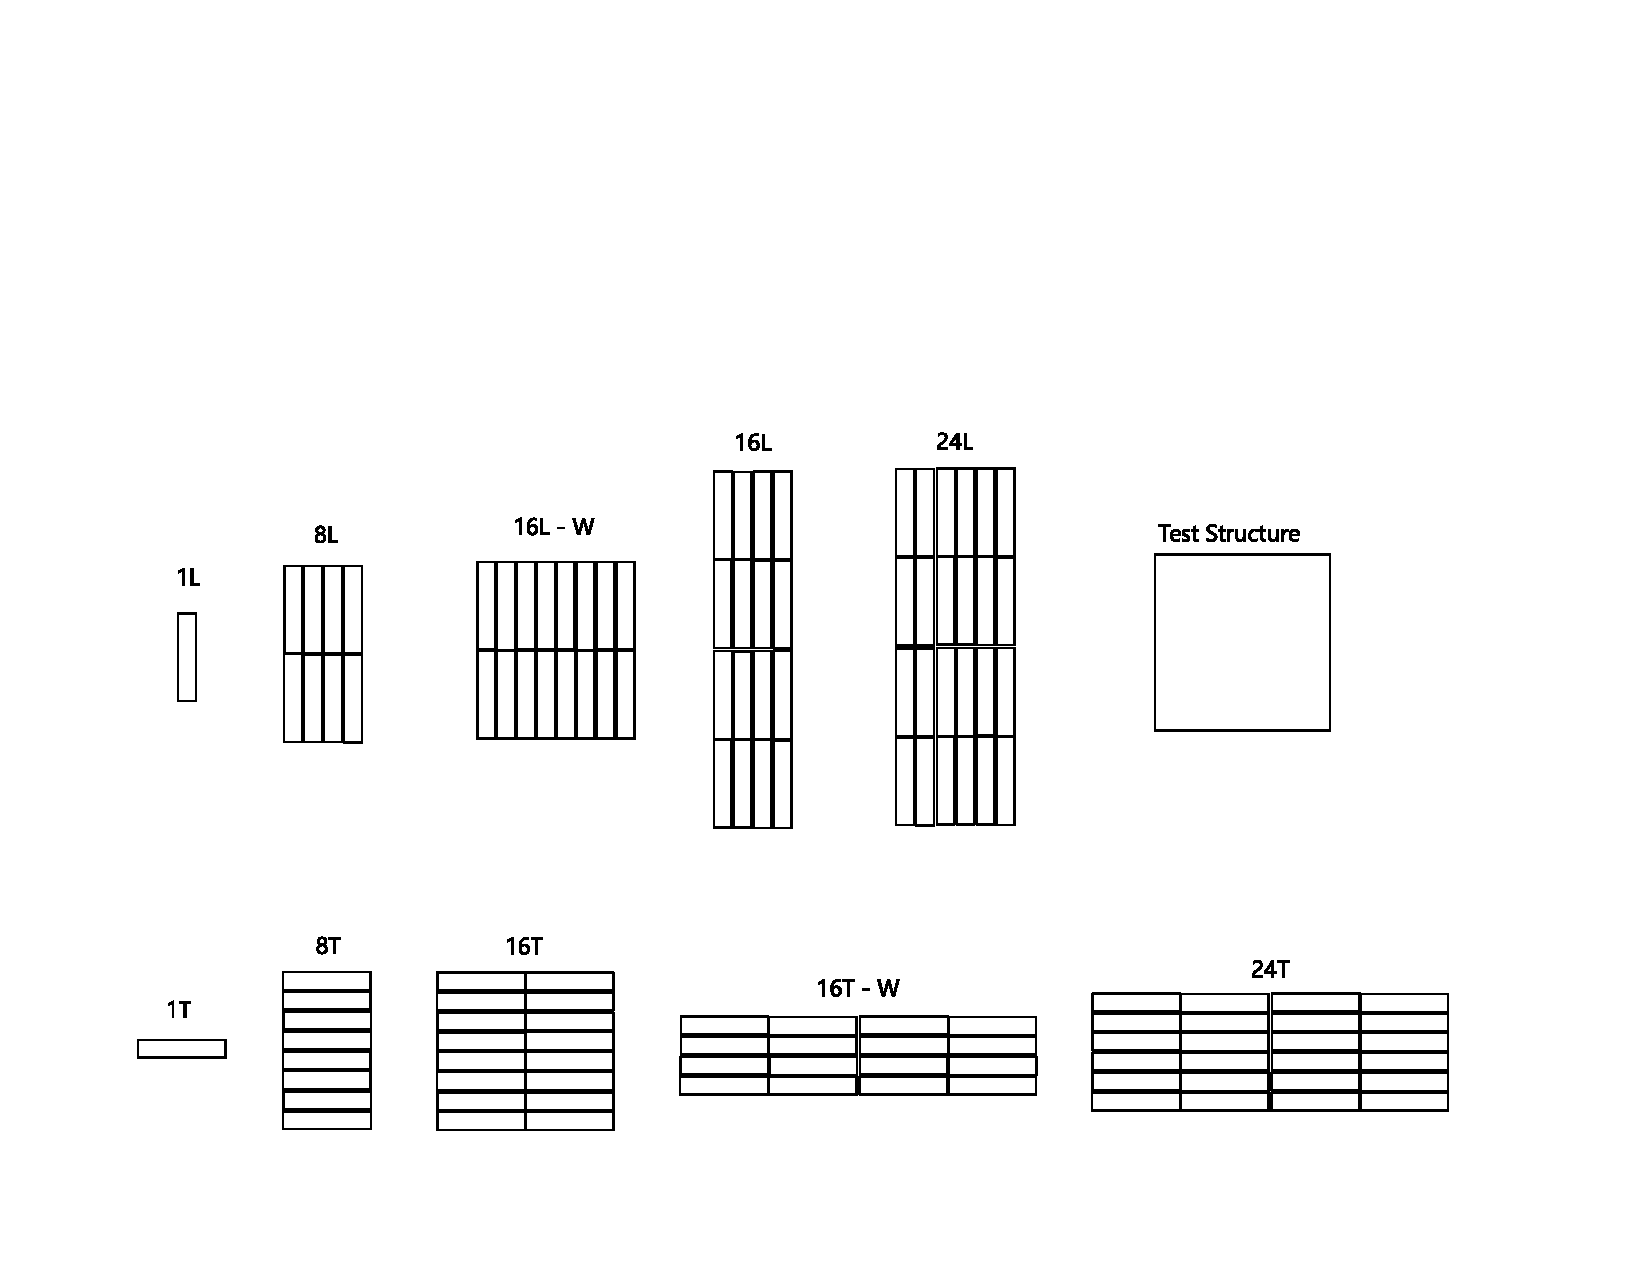
\includegraphics[width=0.8\textwidth]{Configurations.jpg}
    \caption{Regular configurations.}
    \label{fig:configurations}
\end{figure}

\begin{figure}[htbp]
    \centering
    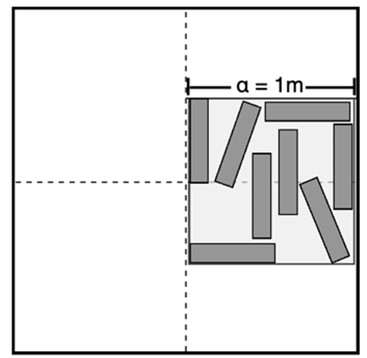
\includegraphics[width=0.48\textwidth]{configurations_rand.jpg}
    \caption{Random configurations.}
    \label{fig:configurations_random}
\end{figure}

\section{Testing Methodology}
\begin{itemize}
    \item Experiments were conducted in a tsunami flume equipped with a rigid mid-flume structure.
    \item Two wave types were tested: unbroken solitary waves and broken solitary waves. This paper focuses on the unbroken solitary wave tests. 
    \item Debris fields were generated in three configurations:
    \begin{itemize}
        \item Regular longitudinal (aligned with flow).
        \item Regular transverse (perpendicular to flow).
        \item Random (both single-size and multi-size).
    \end{itemize}
    \item Force records were decomposed using Butterworth filters:
    \begin{itemize}
        \item High-pass filtering to isolate short-duration impact peaks (Fig.~\ref{fig:high_low_pass}).
        \item Low-pass filtering to capture long-duration damming forces (Fig.~\ref{fig:high_low_pass}).
    \end{itemize}
\end{itemize}

\begin{figure}[htbp]
    \centering
    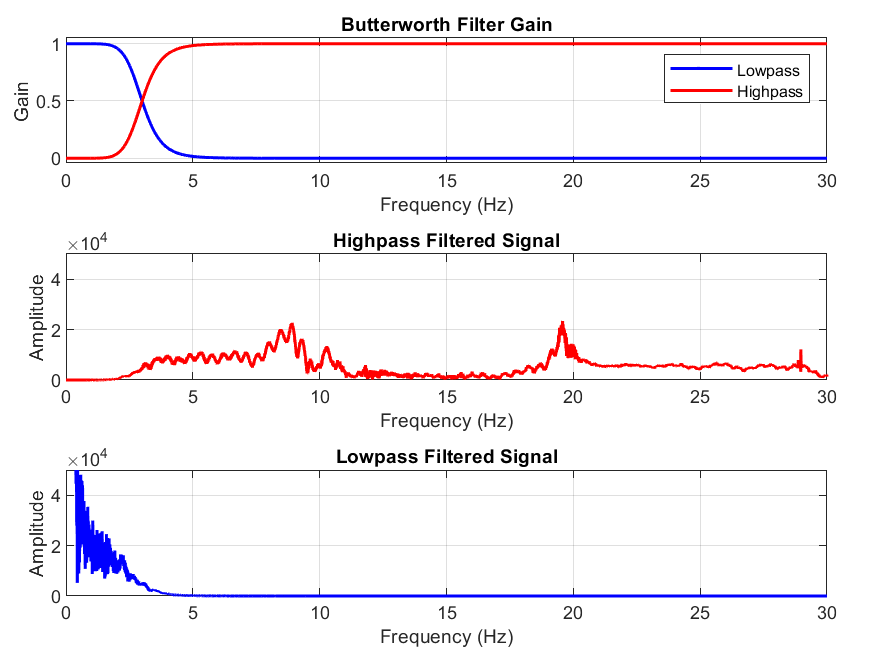
\includegraphics[width=0.8\textwidth]{high_low_pass.png}
    \caption{Force decomposition using Butterworth filters.}
    \label{fig:high_low_pass}
\end{figure}

\begin{figure}[h!]
    \centering
    \begin{subfigure}[b]{0.48\textwidth}
        \centering
        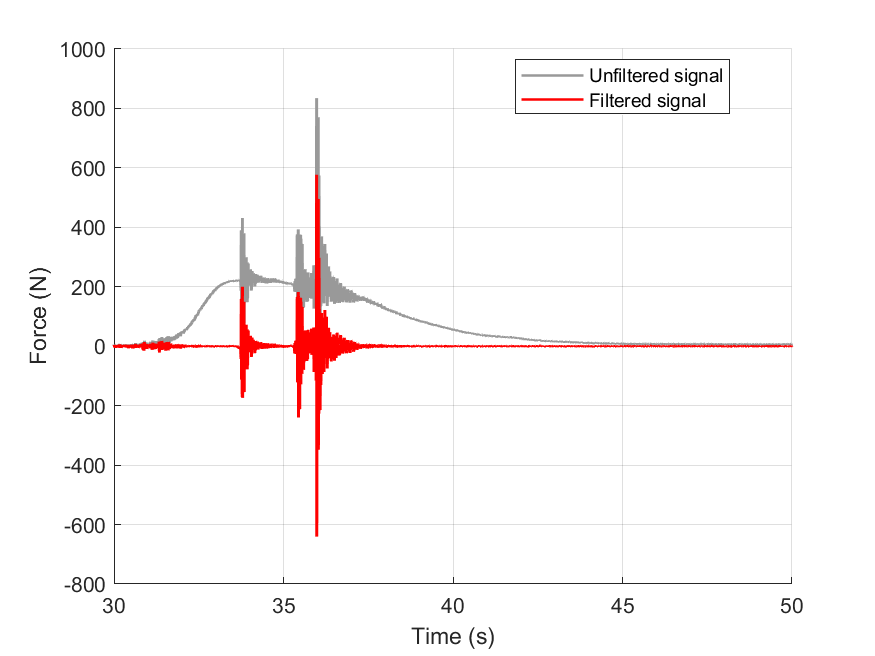
\includegraphics[width=\textwidth]{Reg_Lift_U_1_L_D__Masters_NHERIDeprisImpact2_goodtests_Reg_Lift_U_1_L_Trial04_Peak.png}
        \caption{Force time history for 1L debris.}
        \label{fig:timehist_1L_peak}
    \end{subfigure}
    \hfill
    \begin{subfigure}[b]{0.48\textwidth}
        \centering
        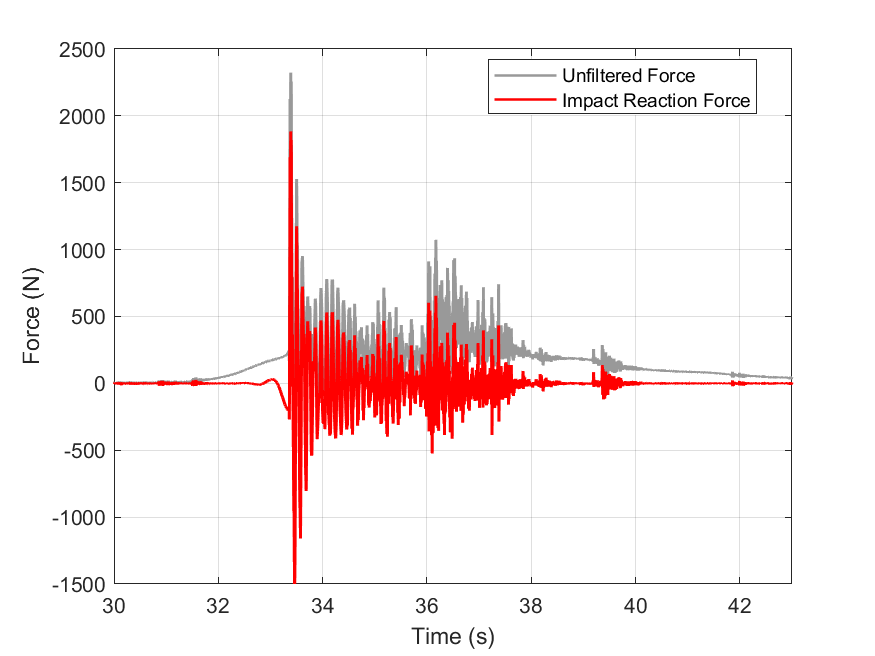
\includegraphics[width=\textwidth]{Reg_Lift_U_24_L_D__Masters_NHERIDeprisImpact2_goodtests_Reg_Lift_U_24_L_Trial04_Peak.png}
        \caption{Force time history for 24L debris.}
        \label{fig:timehist_24L_peak}
    \end{subfigure}
    \caption{Force time histories for (a) 1L debris and (b) 24L debris.}
    \label{fig:timehist_combined}
\end{figure}

\begin{figure}[h!]
    \centering
    \begin{subfigure}[b]{0.48\textwidth}
        \centering
        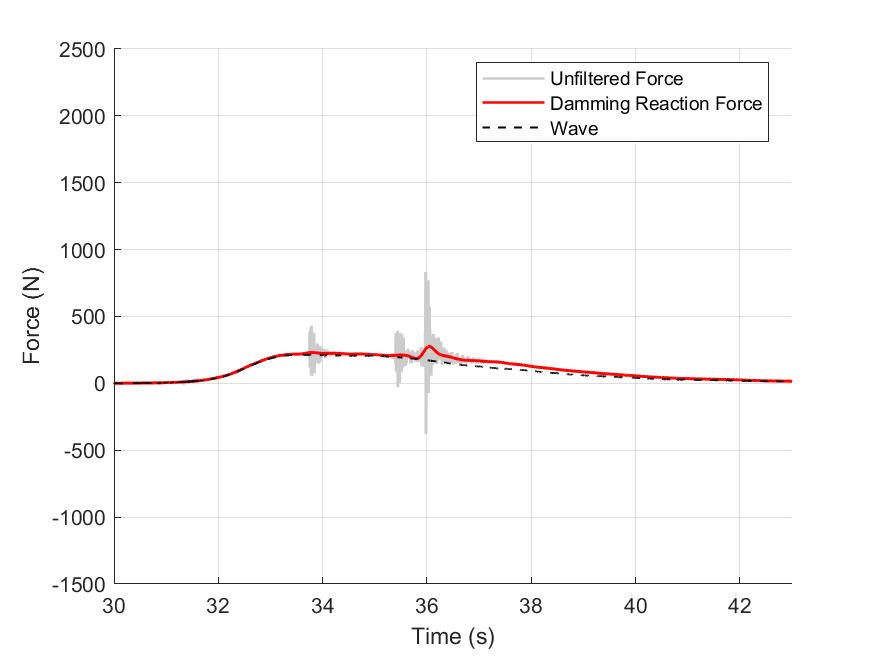
\includegraphics[width=\textwidth]{Reg_Lift_U_1_L_D__Masters_NHERIDeprisImpact2_goodtests_Reg_Lift_U_1_L_Trial04_Damming.png}
        \caption{Damming force time history for 1L debris.}
        \label{fig:timehist_1L_damming}
    \end{subfigure}
    \hfill
    \begin{subfigure}[b]{0.48\textwidth}
        \centering
        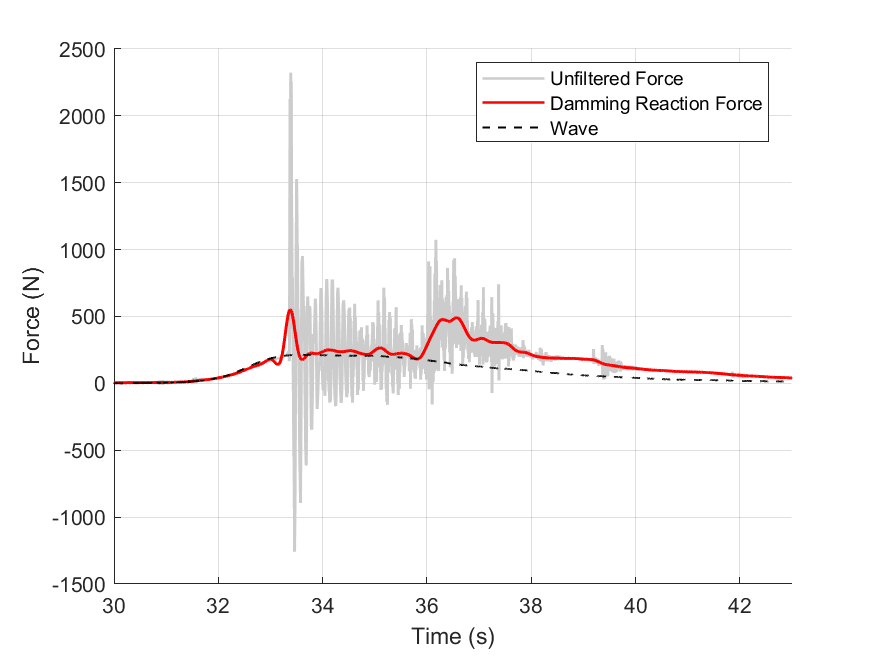
\includegraphics[width=\textwidth]{Reg_Lift_U_24_L_D__Masters_NHERIDeprisImpact2_goodtests_Reg_Lift_U_24_L_Trial04_Damming.png}
        \caption{Damming force time history for 24L debris.}
        \label{fig:timehist_24L_damming}
    \end{subfigure}
    \caption{Damming force time histories for (a) 1L debris and (b) 24L debris.}
    \label{fig:timehist_damming_combined}
\end{figure}


\section{Impact and Damming Reaction forces.}
\begin{itemize}
    \item Video evidence and filtered signals revealed that debris impact occurs in two stages:
    \begin{itemize}
        \item First impact: initial impact on the unsubmerged structure (Fig.~\ref{fig:first_impact}). 
        \item Later impacts: submerged impacts caused by overtopping, suction, and recirculation (Fig.~\ref{fig:second_impact}).
        \item  The first impact is characterized by one simultaneous impact while later impacts show to be more scattered and chaotic especially for high debris numbers (Fig.~\ref{fig:timehist_24L_peak}).
    \end{itemize}
    \item This behavior was consistent across debris types and configurations, highlighting the need to distinguish between first and late peaks.
\end{itemize}

\begin{figure}[htbp]
    \centering
    \begin{subfigure}[b]{0.48\textwidth}
        \centering
        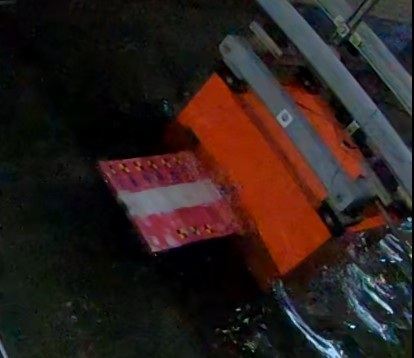
\includegraphics[width=\textwidth]{first_impact.jpg}
        \caption{Initial unsubmerged impact.}
        \label{fig:first_impact}
    \end{subfigure}
    \hfill
    
    \begin{subfigure}[b]{0.48\textwidth}
        \centering
        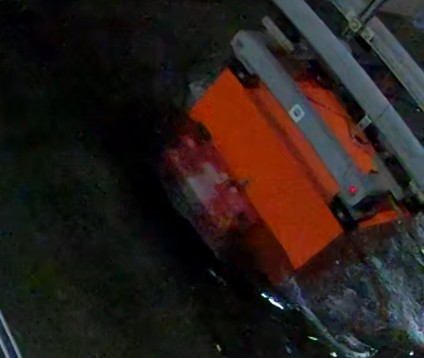
\includegraphics[width=\textwidth]{second_impact.jpg}
        \caption{Later submerged impact.}
        \label{fig:second_impact}
    \end{subfigure}
    \caption{Impact events: (a) initial unsubmerged impact and (b) later submerged impact.}
    \label{fig:impact_combined}
\end{figure}


\section{Results: Impact Reaction Forces}

\subsection{Regular Configurations}
\begin{itemize}
    \item First impact peaks increased linearly with debris number (Fig.~\ref{fig:firstpeak_regular_remap}).
    \item Later impacts showed nonlinear growth, saturating at higher debris counts (Fig.~\ref{fig:laterpeak_regular_remap}).
    \item Longitudinal layouts produced the highest impact forces, while transverse layouts yielded smaller peaks due to water cushioning.
    \item For the 24T and 16T2 tests, debris field area exceeded the structure area. Only part of the debris contacted the structure, so the data was remapped to reflect the effective area (Figs.~\ref{fig:firstpeak_regular_remap}, \ref{fig:laterpeak_regular_remap}).
    \item Remapping makes the 24T case comparable to a 12T case, the total debris count still altered the flume hydrodynamics. This explains why the remapped forces (e.g., for 24T) appear lower than the corresponding smaller-group tests.

\end{itemize}
\begin{figure}[htbp]
    \centering
    \begin{subfigure}[t]{0.48\textwidth}
        \centering
        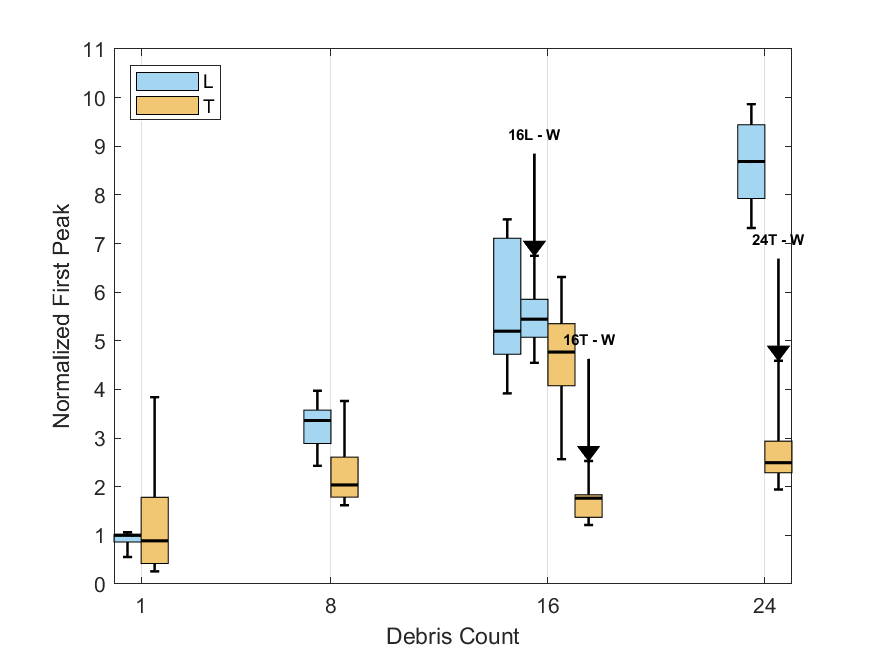
\includegraphics[width=\textwidth]{FirstPeak_Regular_SplitByTrial.png}
        \caption{Original.}
        \label{fig:firstpeak_regular_original}
    \end{subfigure}
    \hfill
    \begin{subfigure}[t]{0.48\textwidth}
        \centering
        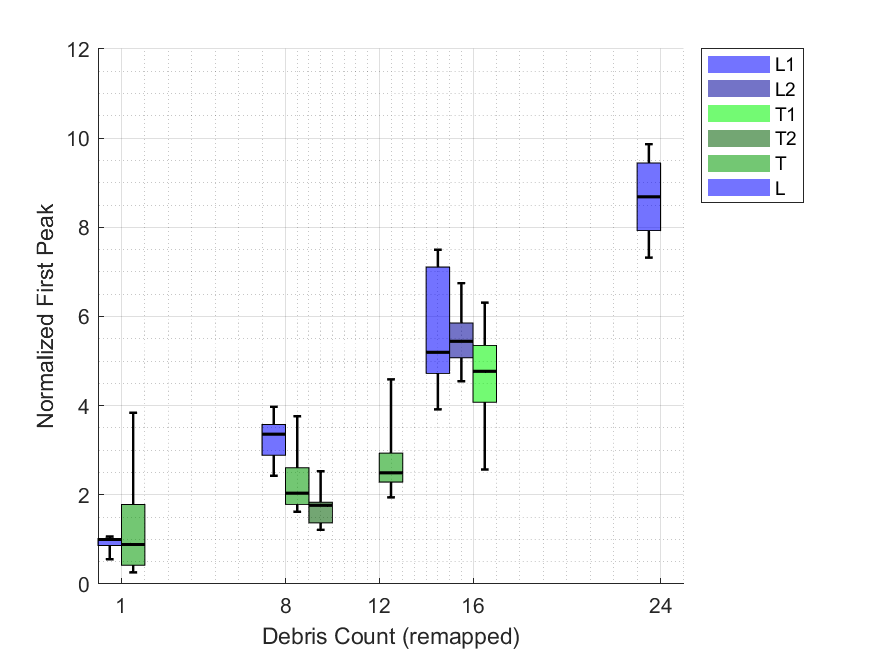
\includegraphics[width=\textwidth]{FirstPeak_Regular_RemappedT.png}
        \caption{Remapped.}
        \label{fig:firstpeak_regular_remap}
    \end{subfigure}
    \caption{First peak forces in regular configurations: (a) original trials, (b) remapped trials.}
    \label{fig:firstpeak_regular_split}
\end{figure}

\begin{figure}[htbp]
    \centering
    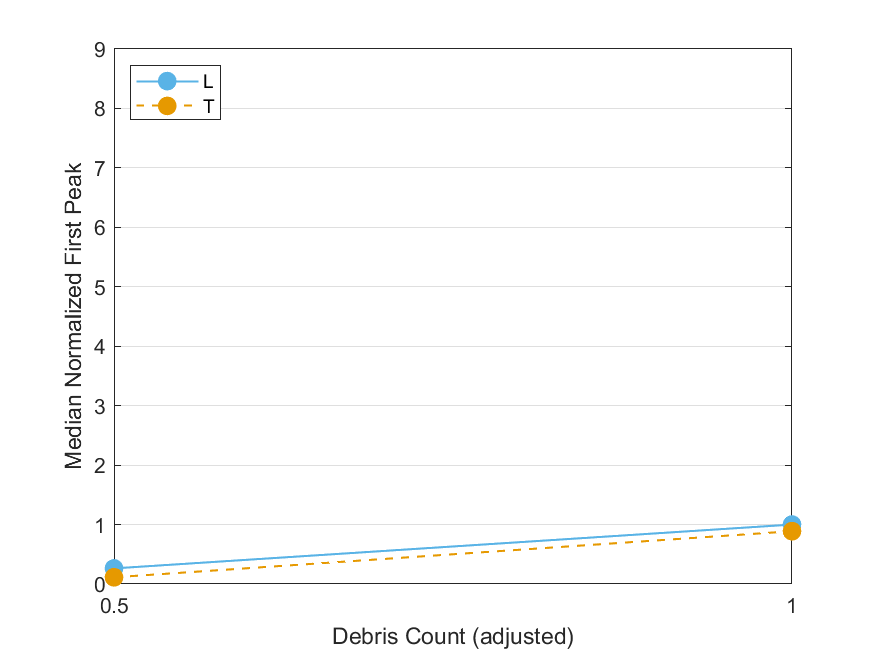
\includegraphics[width=0.8\textwidth]{FirstPeak_Regular_RemappedT_MediansTrend.png}
    \caption{Median normalized first peak values with Wide markers and trend lines.}
    \label{fig:firstpeak_medians_trend}
\end{figure}

% \begin{figure}[htbp]
%     \centering
%     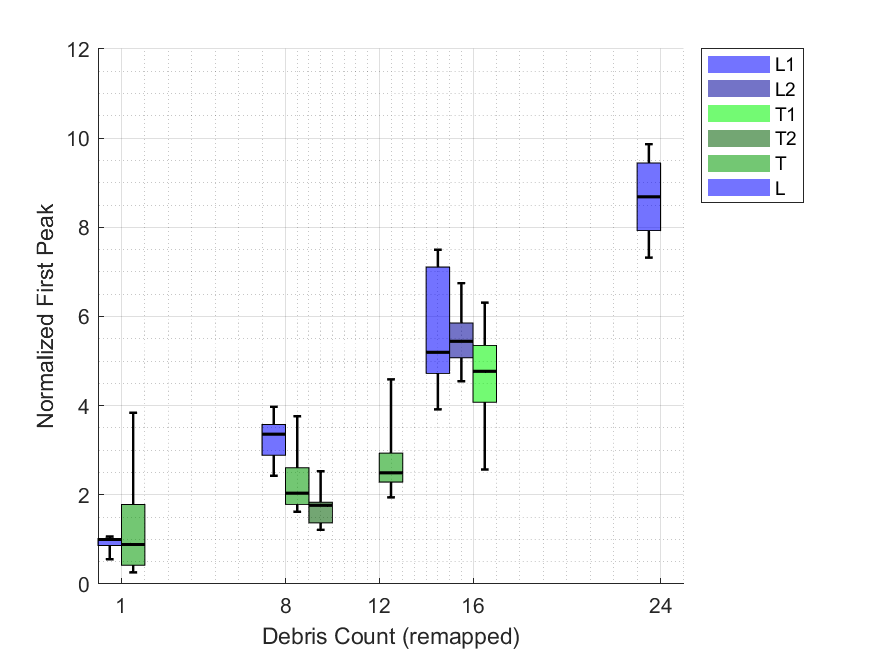
\includegraphics[width=0.8\textwidth]{FirstPeak_Regular_RemappedT.png}
%     \caption{First peak forces in regular configurations (remapped).}
%     \label{fig:firstpeak_regular_remap}
% \end{figure}
\begin{figure}[htbp]
    \centering
    \begin{subfigure}[t]{0.48\textwidth}
        \centering
        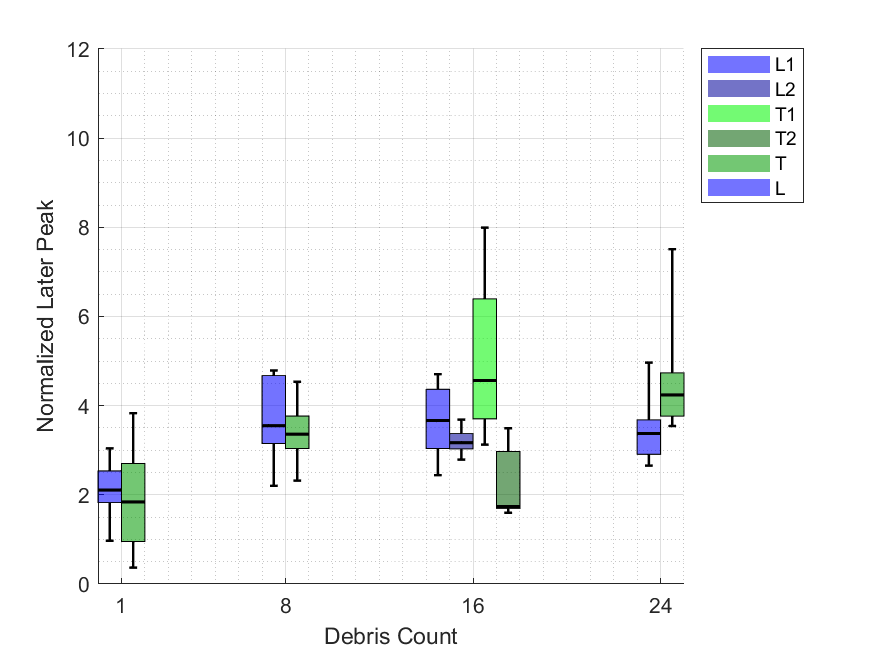
\includegraphics[width=\textwidth]{LaterPeak_Regular_SplitByTrial.png}
        \caption{Original.}
        \label{fig:laterpeak_regular_original}
    \end{subfigure}
    \hfill
    \begin{subfigure}[t]{0.48\textwidth}
        \centering
        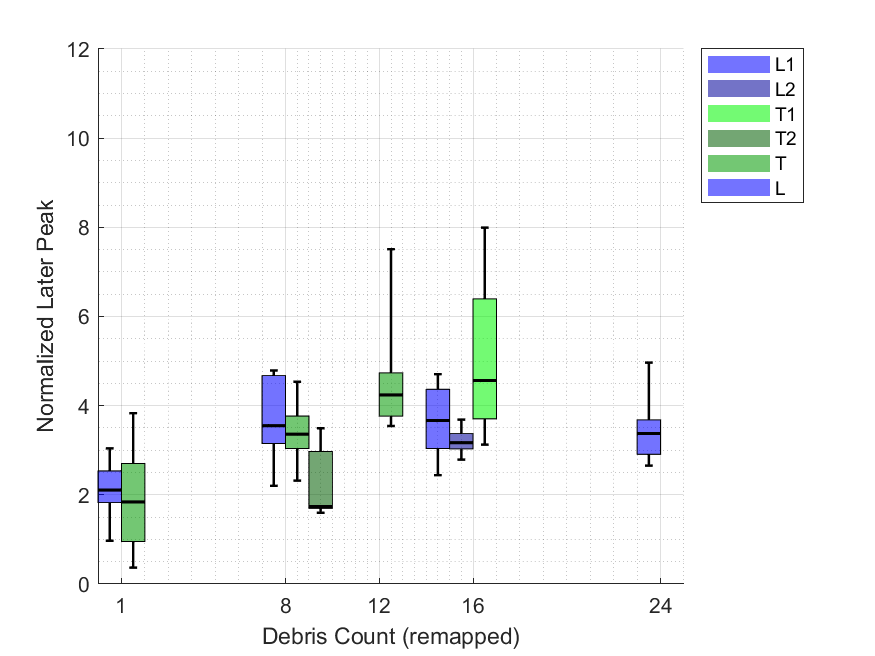
\includegraphics[width=\textwidth]{LaterPeak_Regular_RemappedT.png}
        \caption{Remapped.}
        \label{fig:laterpeak_regular_remap}
    \end{subfigure}
    \caption{Later peak forces in regular configurations: (a) original trials, (b) remapped trials.}
    \label{fig:laterpeak_regular_split}
\end{figure}

\begin{figure}[htbp]
    \centering
    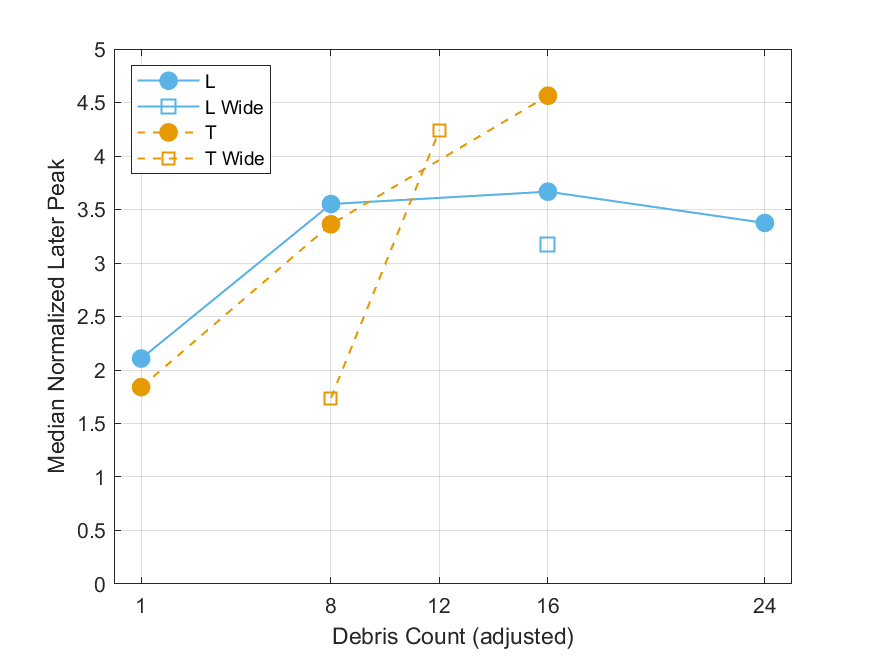
\includegraphics[width=0.8\textwidth]{LaterPeak_Regular_RemappedT_MediansTrend.png}
    \caption{Median normalized later peak values with Wide markers and trend lines.}
    \label{fig:laterpeak_medians_trend}
\end{figure}

% \begin{figure}[htbp]
%     \centering
%     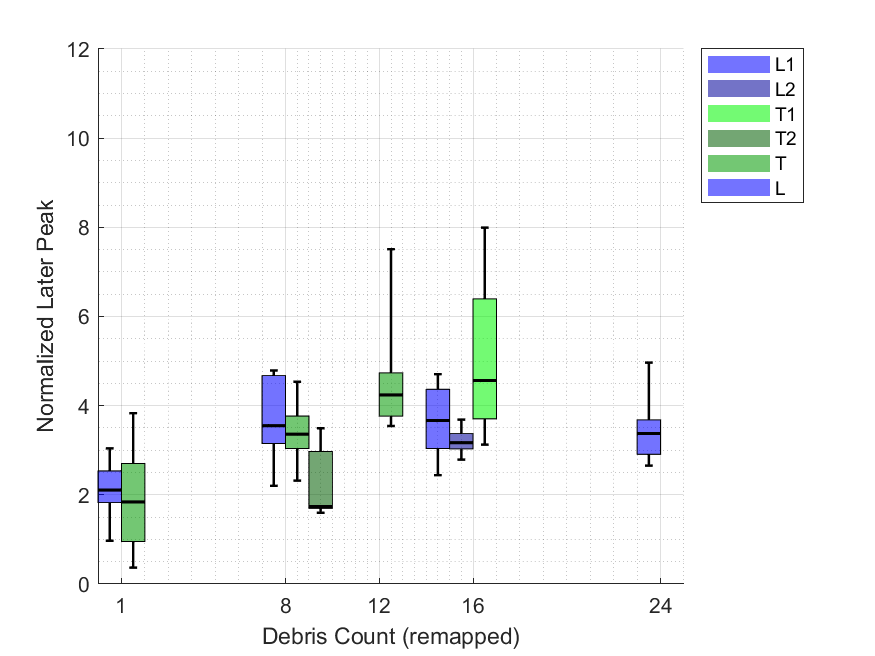
\includegraphics[width=0.8\textwidth]{LaterPeak_Regular_RemappedT.png}
%     \caption{Later peak forces in regular configurations (remapped).}
%     \label{fig:laterpeak_regular_remap}
% \end{figure}

\subsection{Random Configurations}
\begin{itemize}
    \item Random debris fields produced more scattered and generally smaller peaks compared to regular configurations. The overall variability of the data increased (Fig.~\ref{fig:random_peaks_first}). 
    \item Multi-size fields consistently yielded lower impact magnitudes because smaller blocks contributed less momentum (Figs.~\ref{fig:random_peaks_first}, \ref{fig:boxplot_8}, \ref{fig:boxplot_16}, \ref{fig:boxplot_24}). Multi-impact vs.\ single-impact scenarios became more relevant with larger debris groups, as multiple smaller blocks often struck separately rather than together.
    \item The influence of surface area density was critical in impact likelihood and synchronization:
    \begin{itemize}
        \item At low debris counts (e.g., 8 pieces), differences between densities were minimal, since the debris did not spread widely enough across the flume to significantly alter impact probability (Fig.~\ref{fig:boxplot_8}).
        \item At higher counts (16 and 24 pieces), debris were forced to span the full flume width. This spreading meant that not all blocks could align with the structure, reducing the chance of simultaneous impacts.
        \item As density increased in these larger groups, more blocks were able to cluster in front of the structure, increasing the probability of impact and producing stronger peaks (Figs.~\ref{fig:boxplot_16}, \ref{fig:boxplot_24}).
        \item The resulting trends were nonlinear: adding more debris did not guarantee higher peaks, since dispersion could offset the momentum contribution of additional blocks.
    \end{itemize}
\end{itemize}

\begin{figure}[htbp]
    \centering
    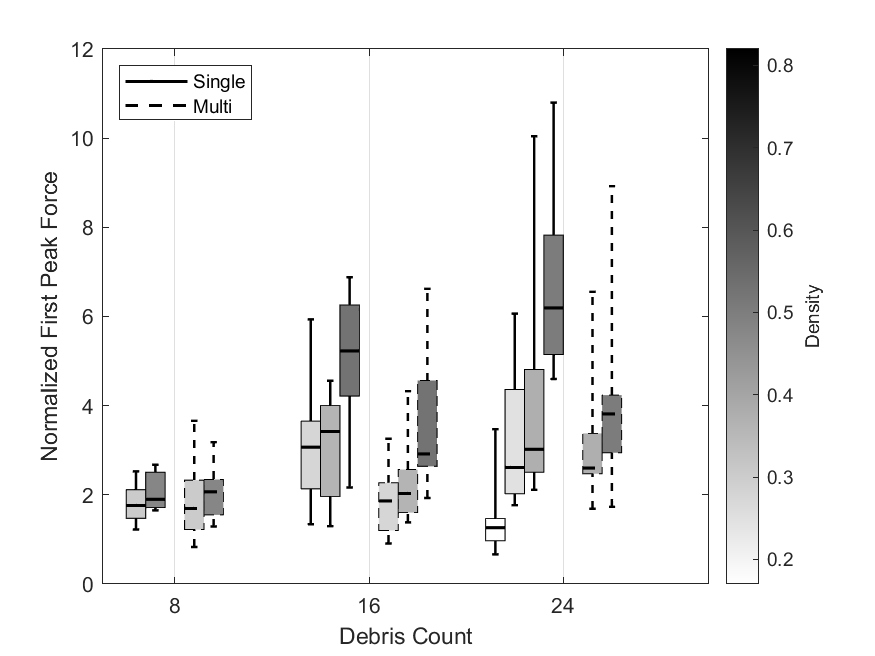
\includegraphics[width=0.8\textwidth]{First_Peak_Random_Single_vs_Multi_ByDensityGradient.png}
    \caption{First impact forces in random fields.}
    \label{fig:random_peaks_first}
\end{figure}

\begin{figure}[htbp]
    \centering
    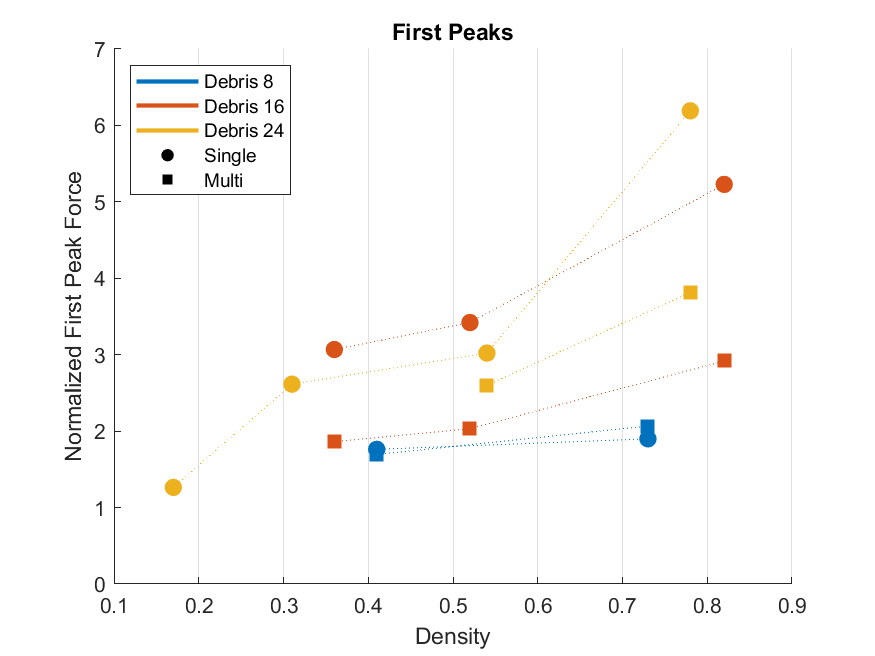
\includegraphics[width=0.7\textwidth]{Impact_FirstPeaks_densities_combined.png}
    \caption{First impact peaks. }
    \label{fig:first_peaks_combined}
\end{figure}

\begin{figure}[htbp]
    \centering
    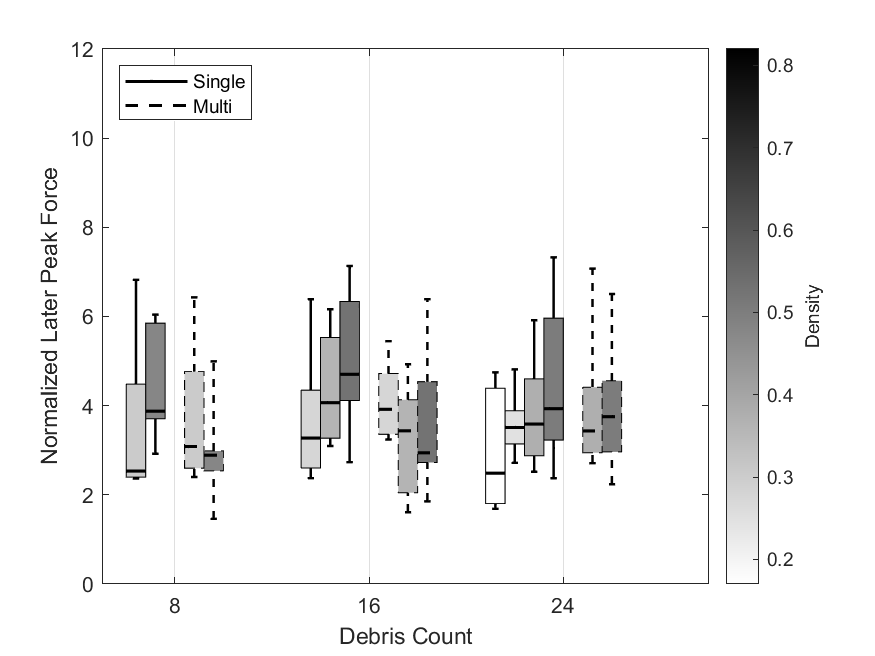
\includegraphics[width=0.8\textwidth]{Later_Peak_Random_Single_vs_Multi_ByDensityGradient.png}
    \caption{Later impact forces in random fields.}
    \label{fig:random_peaks_later}
\end{figure}


\begin{figure}[htbp]
    \centering
    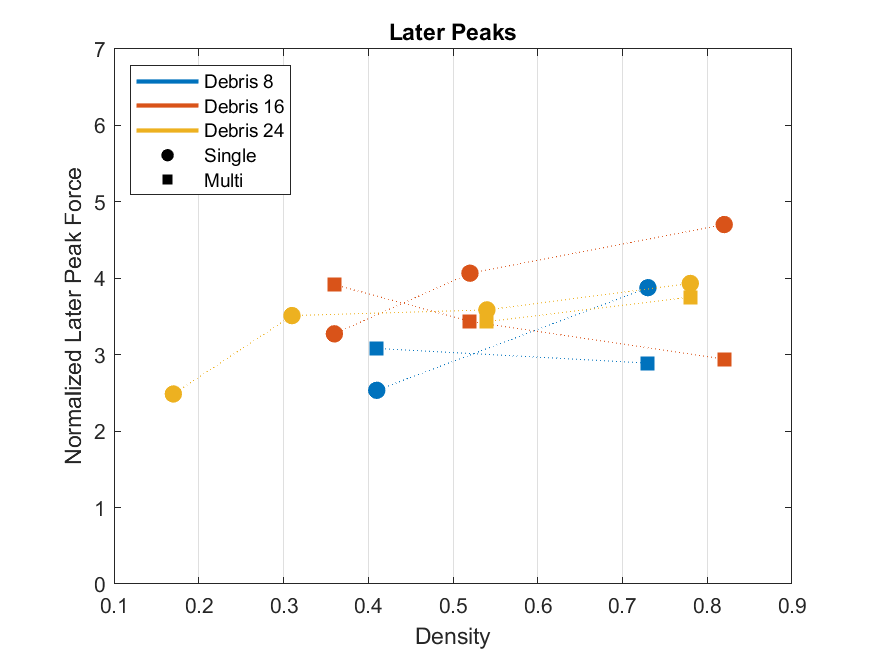
\includegraphics[width=0.7\textwidth]{Impact_LaterPeaks_densities_combined.png}
    \caption{Later impact peaks.}
    \label{fig:later_peaks_combined}
\end{figure}

\begin{figure}[htbp]
    \centering
    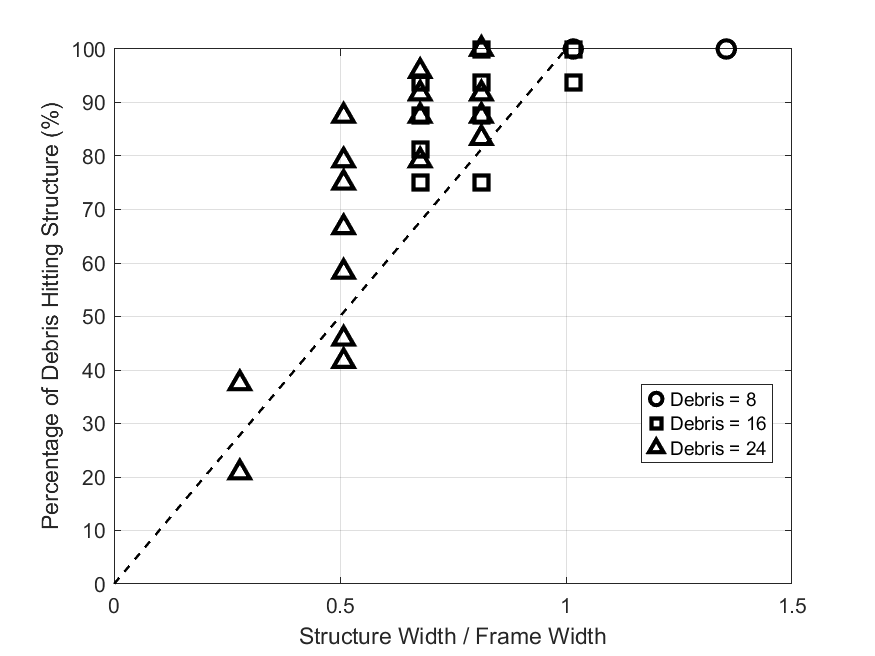
\includegraphics[width=0.8\textwidth]{Impact_probabilities.png}
    \caption{Impact probabilities across random trials.}
    \label{fig:impact_probabilities}
\end{figure}


\section{Results: Damming Reaction Forces}
\begin{itemize}
    \item Damming forces, extracted by low-pass filtering, reflected sustained blockage (Figs.~\ref{fig:damming_regular_remap}, \ref{fig:damming_random}).
    \item Single-size debris: increasing density led to stable jams and higher damming loads, as expected from tighter packing and reduced bypassing flow.
    \item Multi-size debris: smaller blocks prevented stable blockages, keeping forces lower and making density effects minimal (Fig.~\ref{fig:damming_random}).
    \item Longitudinal vs.\ transverse: while the overall magnitudes were comparable, transverse cases produced higher damming loads once debris counts exceeded eight. This supports the broader trend that longitudinal configurations dominate impact peaks, while transverse configurations dominate damming.
    \item Nonlinear behavior was observed, with damming forces saturating at higher debris counts. This parallels the nonlinear growth seen in the later submerged impact stage. This saturation is partly due to the complete blockage being achieved and partly due to debris pieces recirculating.
\end{itemize}

% According to \cite{bonusEvaluationFluidDrivenDebris}, 
\begin{figure}[htbp]
    \centering
    \begin{subfigure}[t]{0.48\textwidth}
        \centering
        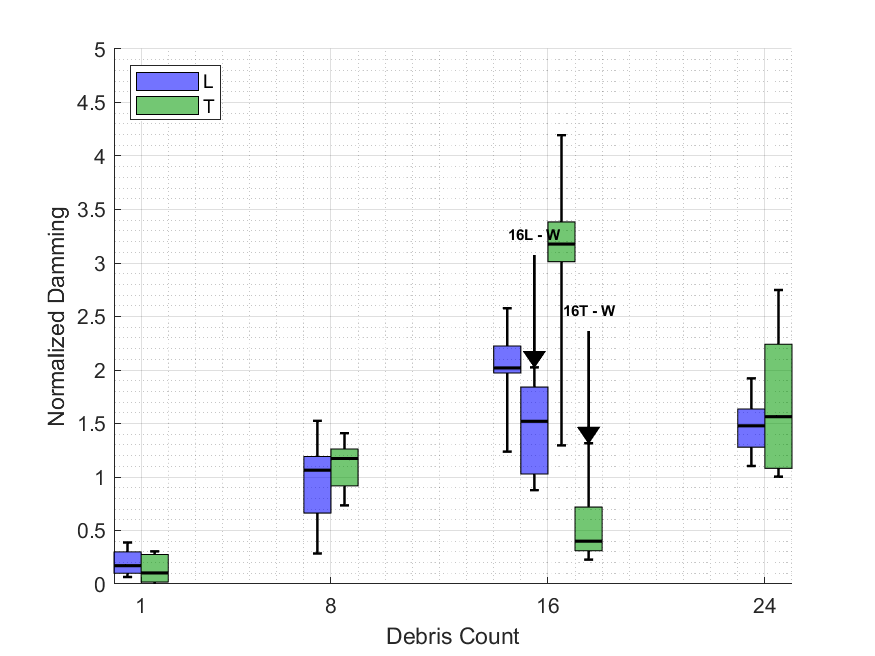
\includegraphics[width=\textwidth]{Damming_Regular_SplitByTrial.png}
        \caption{Original.}
        \label{fig:damming_regular_original}
    \end{subfigure}
    \hfill
    \begin{subfigure}[t]{0.48\textwidth}
        \centering
        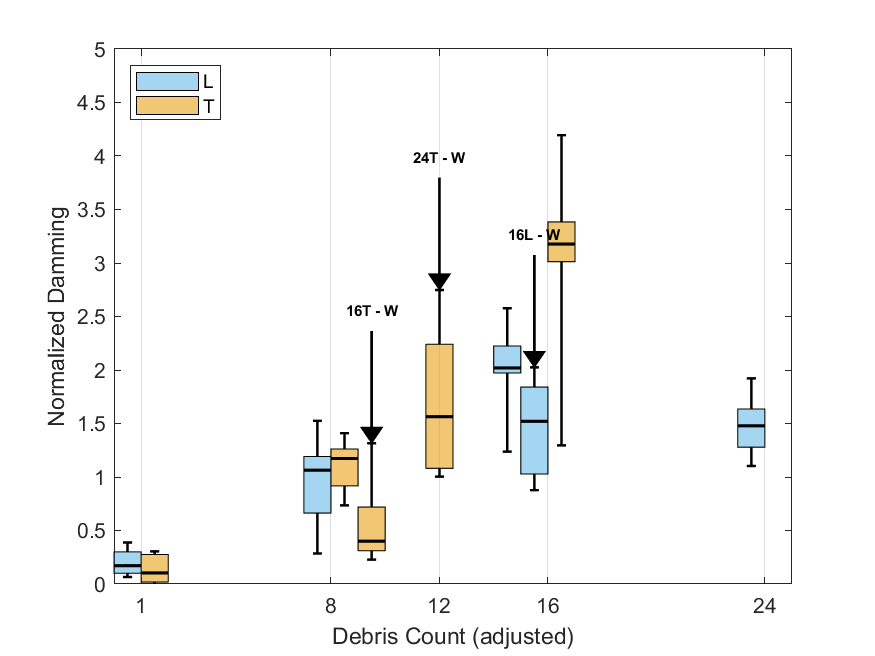
\includegraphics[width=\textwidth]{Damming_Regular_L_T_SplitByTrial_Remapped.png}
        \caption{Remapped.}
        \label{fig:damming_regular_remap}
    \end{subfigure}
    \caption{Damming forces in regular configurations: (a) original trials, (b) remapped trials.}
    \label{fig:damming_regular_split}
\end{figure}

\begin{figure}[htbp]
    \centering
    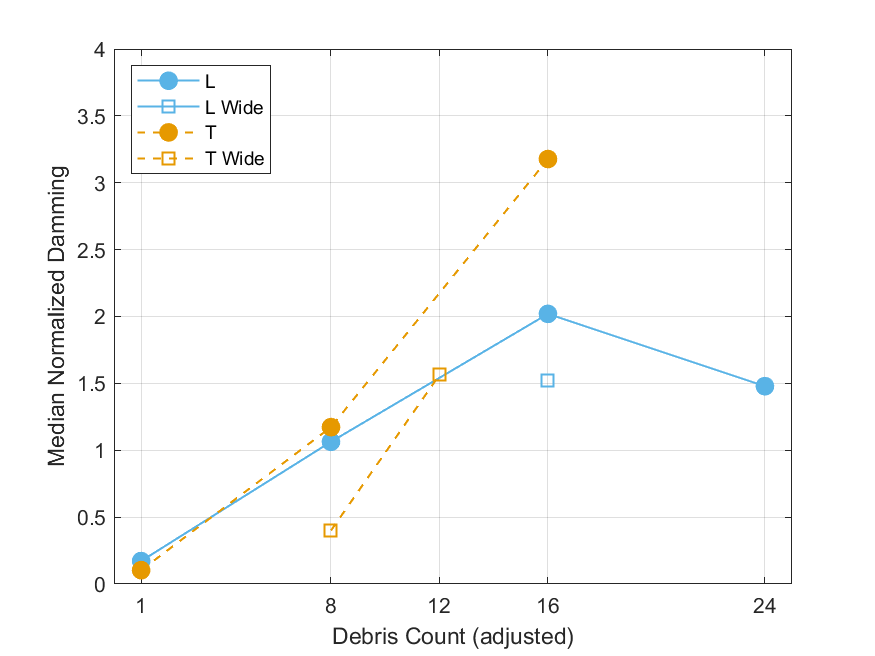
\includegraphics[width=0.8\textwidth]{Damming_Regular_RemappedT_Medians.png}
    \caption{Median normalized damming forces for regular trials with Wide markers.}
    \label{fig:damming_medians_wide}
\end{figure}

% \begin{figure}[htbp]
%     \centering
%     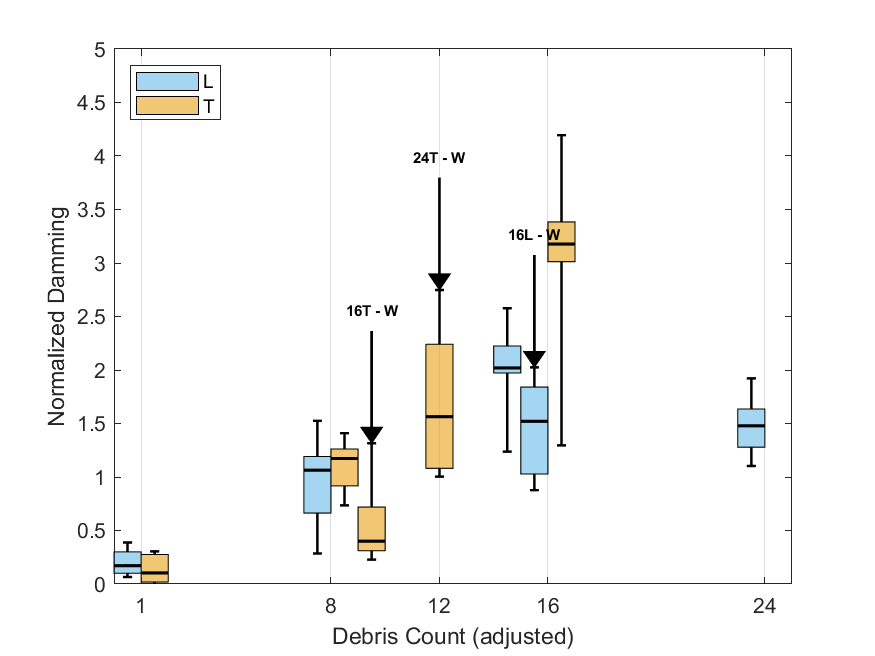
\includegraphics[width=0.8\textwidth]{Damming_Regular_L_T_SplitByTrial_Remapped.png}
%     \caption{Damming forces in regular configurations.}
%     \label{fig:damming_regular_remap}
% \end{figure}

\begin{figure}[htbp]
    \centering
    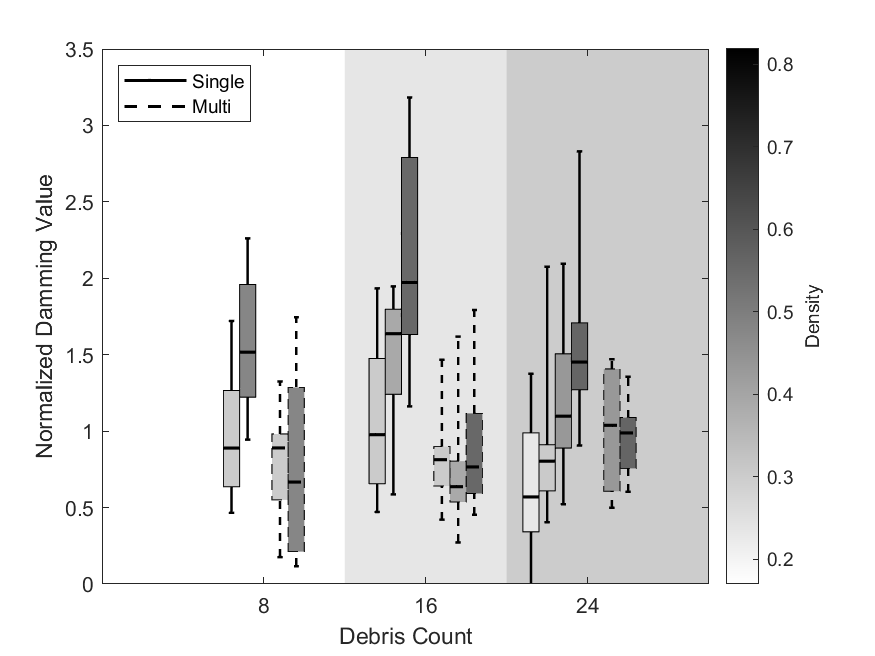
\includegraphics[width=0.8\textwidth]{Damming_Random_Single_vs_Multi_ByDensityGradient.png}
    \caption{Normalized damming forces in random debris fields, separated by Single and Multi debris configurations.}
    \label{fig:random_damming_gradient}
\end{figure}
\begin{figure}[htbp]
    \centering
    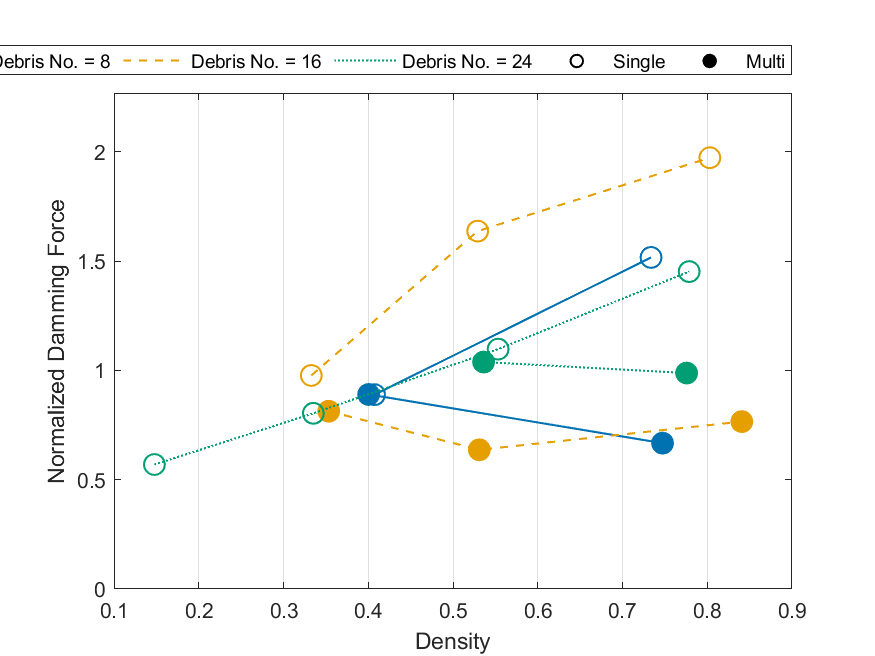
\includegraphics[width=0.6\textwidth]{figures/Damming_Peaks_densities_combined.png}
    \caption{Normalized damming .}
    \label{fig:damming_peaks}
\end{figure}


% \section{Flow Velocities}
% The mean flow velocity in the flume was confirmed to be XYZ. 

\section{Conclusions}
\begin{itemize}
    \item Longitudinal debris groups generated the largest impact peaks, while transverse groups dominated damming loads.
    \item Random and multi-size fields produced smaller and more variable forces.
    \item Surface area density strongly influenced impact probability once debris spread exceeded structure width.
    \item For 24T and 16T2 trials, partial contact required remapping.
    \item First impacts scaled with debris count, while later impacts saturated at higher counts.
    \item Multi-size fields weakened damming loads due to disrupted jamming.
\end{itemize}

\section{Limitations}
\begin{itemize}
    \item Due to high impact forces, loading could not be recorded at the front of the flume. All measured forces are reaction forces and include structural vibrations.
    \item Flume geometry amplified some effects, such as water cushioning, as flow was obstructed by the side walls.
    \item The relative width of debris and structure limited the representativeness of some tests.
    \item Practical limits on debris quantity constrained the range of tested cases.
\end{itemize}
\section{References}
\bibliographystyle{plain}  % or abbrv, alpha, apa, ieee, etc.
\bibliography{Thesis}  % matches your .bib file name

\end{document}
